\documentclass[mathserif]{beamer}
%\usetheme[secheader]{pecostalk}
\graphicspath{{figs/}}
\usepackage{xcolor}


% presentation slides 

\date[12/2/2014]{December 2nd, 2014}
\author[Malaya]{Nicholas Malaya}
\institute{Institute for Computational Engineering and Sciences \\ The University of Texas at Austin}
\title[STC-Project]{C++ implementation of the Metropolis-Hasting Algorithm}

\begin{document}

%===============================================================================
% Title page
\begin{frame}
%
\titlepage
\end{frame}

%===============================================================================
%   Uses of MCMC
%===============================================================================
\begin{frame}
\frametitle{Motivation}

\begin{block}{Extending MC}
  \begin{itemize}
  \item We discussed Monte-Carlo (MC) methods in class
  \item But we can do better-- Markov Chain Monte-Carlo (MCMC) is an extension of MC
  \end{itemize}
\end{block}

\begin{block}{MCMC is ubiquitous}
  \begin{itemize}
  \item statistics, physics, chemistry, biology, engineering, business, linguistics, etc. 
  \item Especially research: Machine Learning, Uncertainty Quantification, Astrophysics, Particle Physics, Risk assessment
  \item \textcolor{blue}{Primarily used for calculating numerical approximations of multi-dimensional integrals}
  \end{itemize}
\end{block}

\end{frame}

%===============================================================================
%     MCMC -- what is it?
%===============================================================================
\begin{frame}
\frametitle{MCMC}

\begin{block}{What is it?}
\begin{itemize}
\item \textcolor{white}{MC}MC = \textcolor{white}{Markov Chain} Monte-Carlo
\item \textcolor{white}{Markov = Each step only depends on previous}
\item \textcolor{white}{Chain = A series of steps}
\item Monte-Carlo = Stochastic (i.e. random numbers)
\end{itemize}
Essentially, a method to generate random \textcolor{white}{steps correlated with the previous step}
\end{block}
\end{frame}

%===============================================================================
%     MCMC -- what is it?
%===============================================================================
\begin{frame}
\frametitle{MCMC}

\begin{block}{What is it?}
\begin{itemize}
\item \textcolor{white}{M}CMC = \textcolor{white}{Markov} Chain Monte-Carlo
\item \textcolor{white}{Markov = Each step only depends on previous}
\item Chain = A series of steps
\item Monte-Carlo = Stochastic (i.e. random numbers)
\end{itemize}
Essentially, a method to generate random steps \textcolor{white}{correlated with the previous step}
\end{block}
\end{frame}

%===============================================================================
%     MCMC -- what is it?
%===============================================================================
\begin{frame}
  \frametitle{MCMC}

  \begin{block}{What is it?}
    \begin{itemize}
    \item \textcolor{black}{M}CMC = \textcolor{black}{Markov} Chain Monte-Carlo
    \item \textcolor{black}{Markov = Each step only depends on previous}
    \item Chain = A series of steps
    \item Monte-Carlo = Stochastic (i.e. random numbers)
    \end{itemize}
    Essentially, a method to generate random steps \textcolor{black}{correlated with the previous step}

  \end{block}
\end{frame}

%===============================================================================
%     Picture Example: reject
%===============================================================================
\begin{frame}
\frametitle{Enter Metropolis-Hastings}

\begin{block}{Intuitive Picture: Sampling a Gaussian Distribution}
  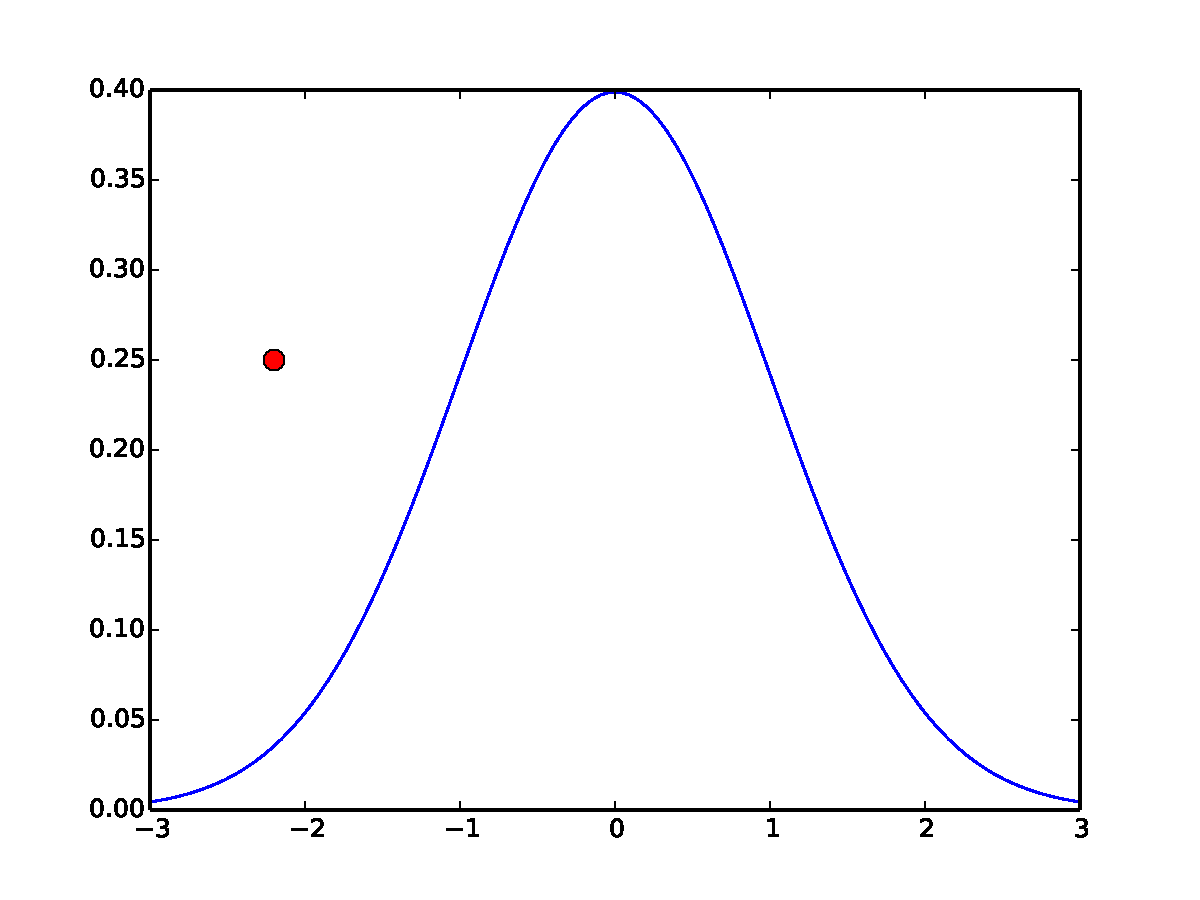
\includegraphics[width=3.5in]{figs/norm.pdf}
\end{block}

\end{frame}

%===============================================================================
%     picture sample one: accept
%===============================================================================
\begin{frame}
\frametitle{Enter Metropolis-Hastings}

\begin{block}{Intuitive Picture: Sampling a Gaussian Distribution}
  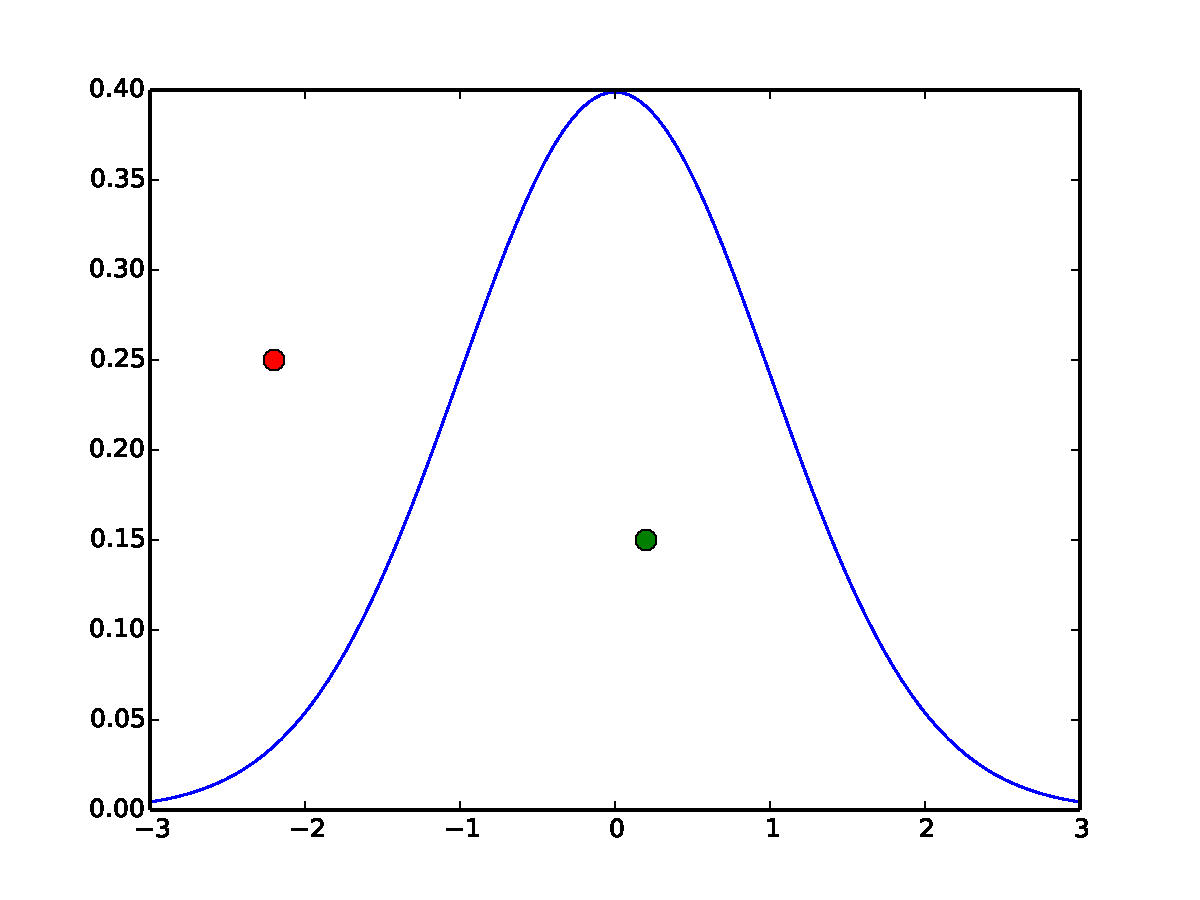
\includegraphics[width=3.5in]{figs/norm-acc.pdf}
\end{block}

\end{frame}

%===============================================================================
%     picture sample one: correlated
%===============================================================================
\begin{frame}
\frametitle{Enter Metropolis-Hastings}

\begin{block}{Intuitive Picture: Sampling a Gaussian Distribution}
  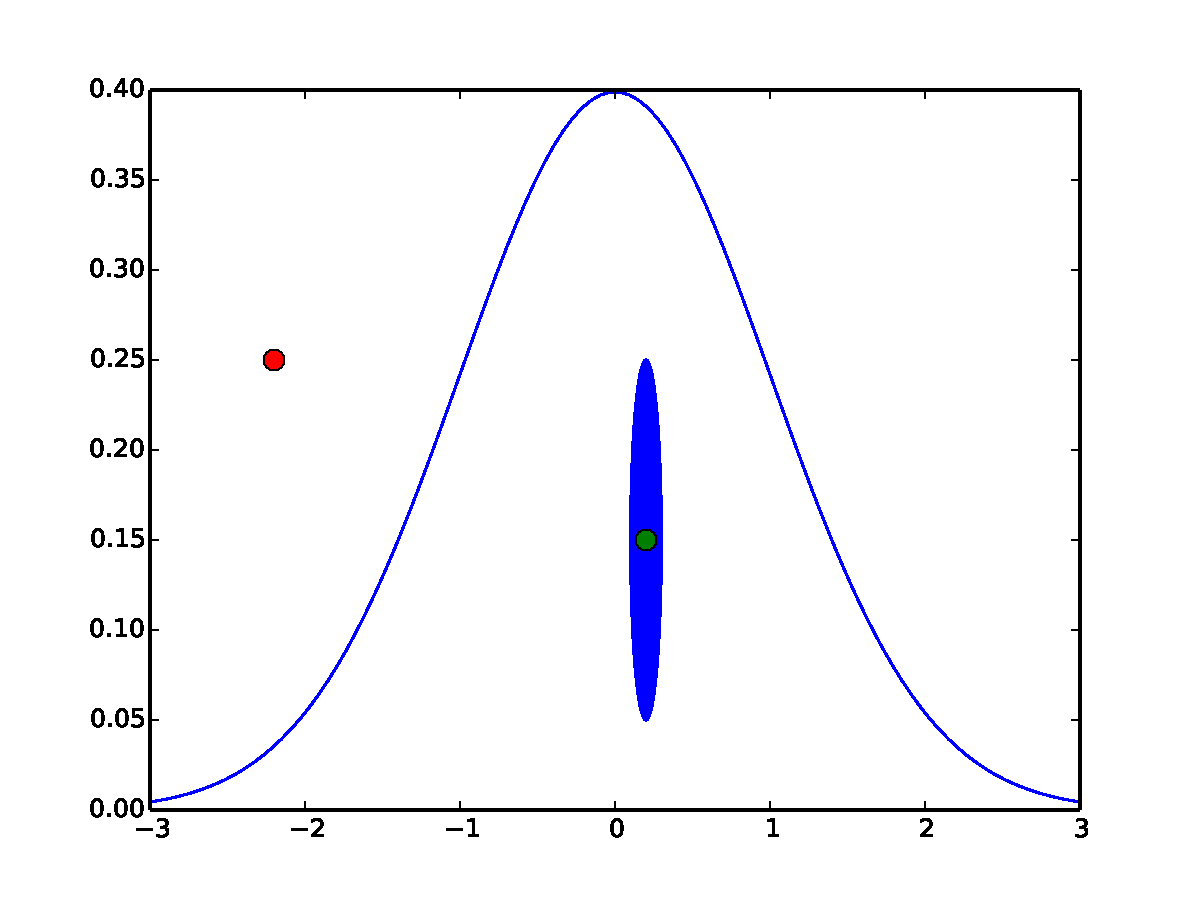
\includegraphics[width=3.5in]{figs/norm-corr.pdf}
\end{block}

\end{frame}


%===============================================================================
%     So... what is metropolis-hastings?
%===============================================================================
\begin{frame}
\frametitle{Enter Metropolis-Hastings}

\begin{block}{What is it?}
  \begin{itemize}
  \item Metropolis-Hastings is an MCMC method for generating these samples. 
  \end{itemize}
\end{block}

\begin{block}{Algorithm}
  \begin{itemize}
  \item Start at current step ($\phi_1$)
  \item Draw proposal: $q(\tilde \phi_2 | \phi_1) = N(\tilde \phi_2 | \phi_1, \nu^2)$
  \item Draw from uniform: $u \sim U(0,1)$
  \item if: $u < \frac{\pi_n(\tilde \phi_2)}{\pi_n(\phi_1)}$ ($\pi_n$ is bayesian posterior, etc.)
    \begin{itemize}
    \item $\phi_2 = \tilde \phi_2$
    \end{itemize}
  \item else: $\phi_2 = \phi_1$
  \end{itemize}
\end{block}

\end{frame}

%===============================================================================
%     So... what is metropolis-hastings?
%===============================================================================
\begin{frame}
\frametitle{Enter Metropolis-Hastings}

\begin{block}{What is it?}
  \begin{itemize}
  \item Metropolis-Hastings is an MCMC method for generating these samples. 
  \end{itemize}
\end{block}

\begin{block}{Algorithm}
  \begin{itemize}
  \item Start at current step ($\phi_1$)
  \item Draw proposal: $q(\tilde \phi_2 | \phi_1) = N(\tilde \phi_2 | \phi_1, \nu^2)$
  \item Draw from uniform: $u \sim U(0,1)$
  \item if: $u < \frac{\pi_n(\tilde \phi_2)}{\pi_n(\phi_1)}$ ($\pi_n$ is bayesian posterior, etc.)
    \begin{itemize}
    \item $\phi_2 = \tilde \phi_2$
    \end{itemize}
  \item else: $\phi_2 = \phi_1$
  \end{itemize}
\end{block}

\textcolor{red}{Question: How do we choose $\nu$?}

\end{frame}

%===============================================================================
%     Results of chain
%===============================================================================
\begin{frame}
  \frametitle{Project Status}

  \begin{block}{Library Snapshot}
    \begin{itemize}
    \item C++, threaded with OpenMP
    \item Makefile build system support for:
      \begin{itemize}
      \item Asus laptop 
      \item TACC's Lonestar supercomputer
      \end{itemize}
    \item Git revision control 
    \item CLOC: 254 SLOC C++
    \end{itemize}
  \end{block}
    
    \begin{block}{Capabilities}
      \begin{itemize}
      \item Gamma, Beta, Normal Statistical Distributions
      \end{itemize}
    \end{block}
      
\end{frame}

%===============================================================================
%     Picture Example: reject
%===============================================================================
\begin{frame}
\frametitle{Metropolis-Hastings Sampling in C++}

\begin{block}{Sampling a Gamma Distribution}
  \begin{columns}
  \column{0.35\textwidth}
    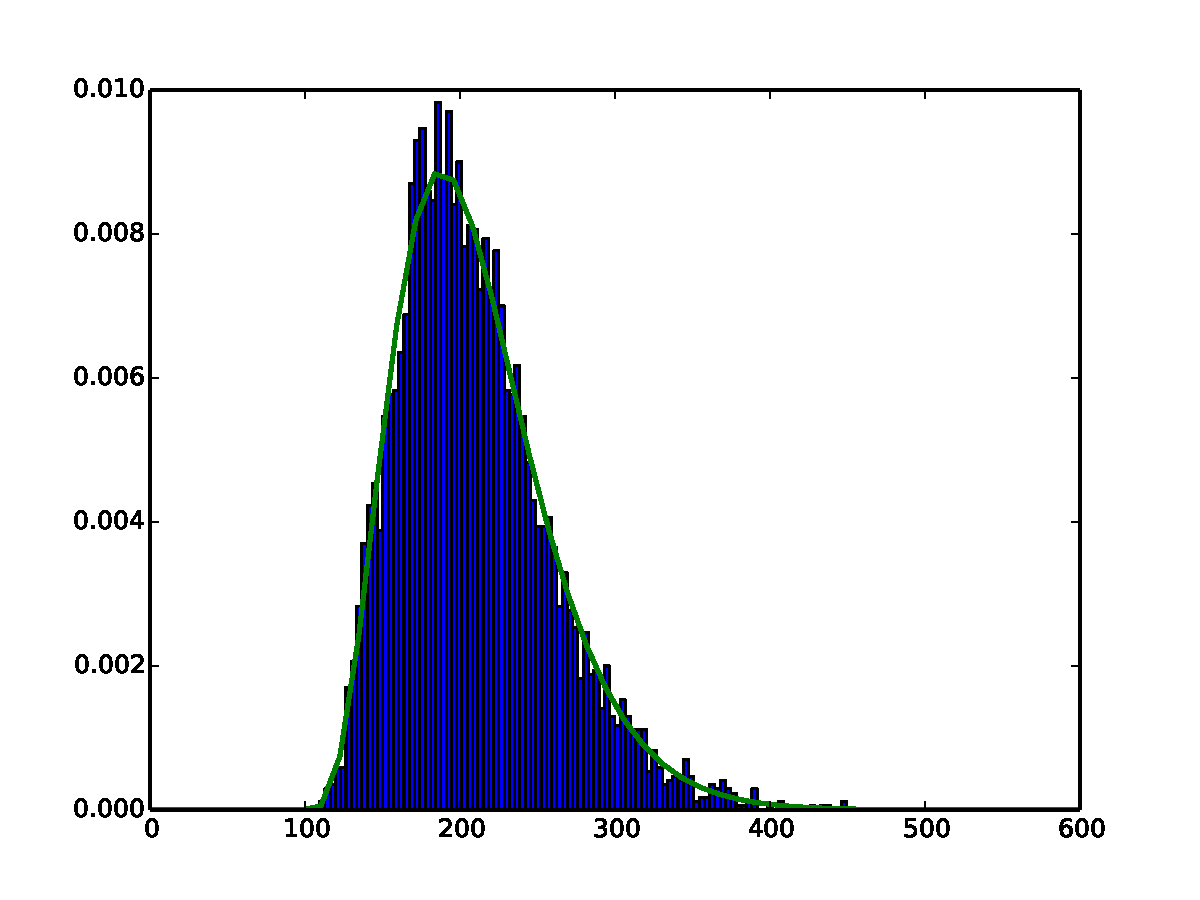
\includegraphics[width=3in]{figs/gamma.pdf}

  \column{0.5\textwidth}
  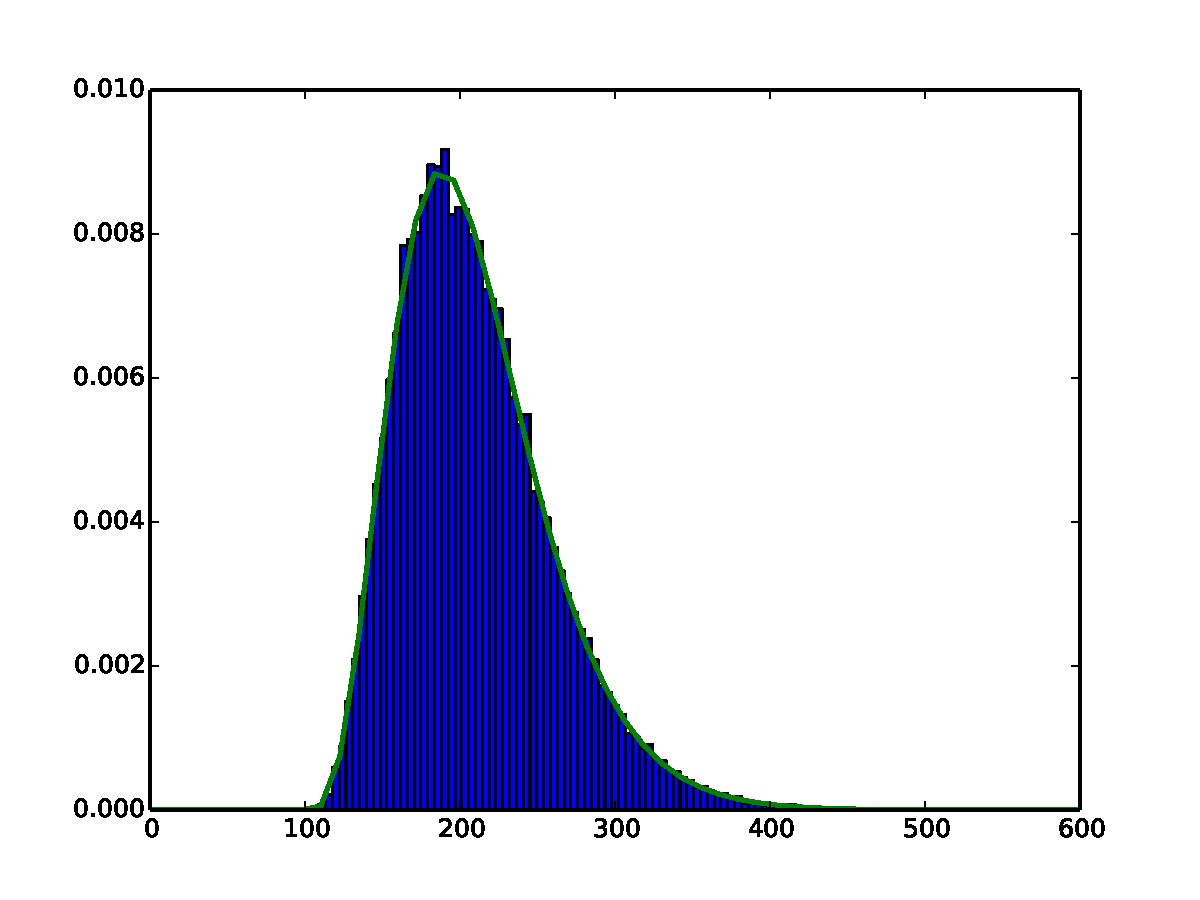
\includegraphics[width=3in]{figs/gamma_50k.pdf}
  \end{columns}
\end{block}

\end{frame}


%===============================================================================
%     OpenMP intro
%===============================================================================
\begin{frame}
\frametitle{Burn-in}

\begin{block}{MCMC Chain}
  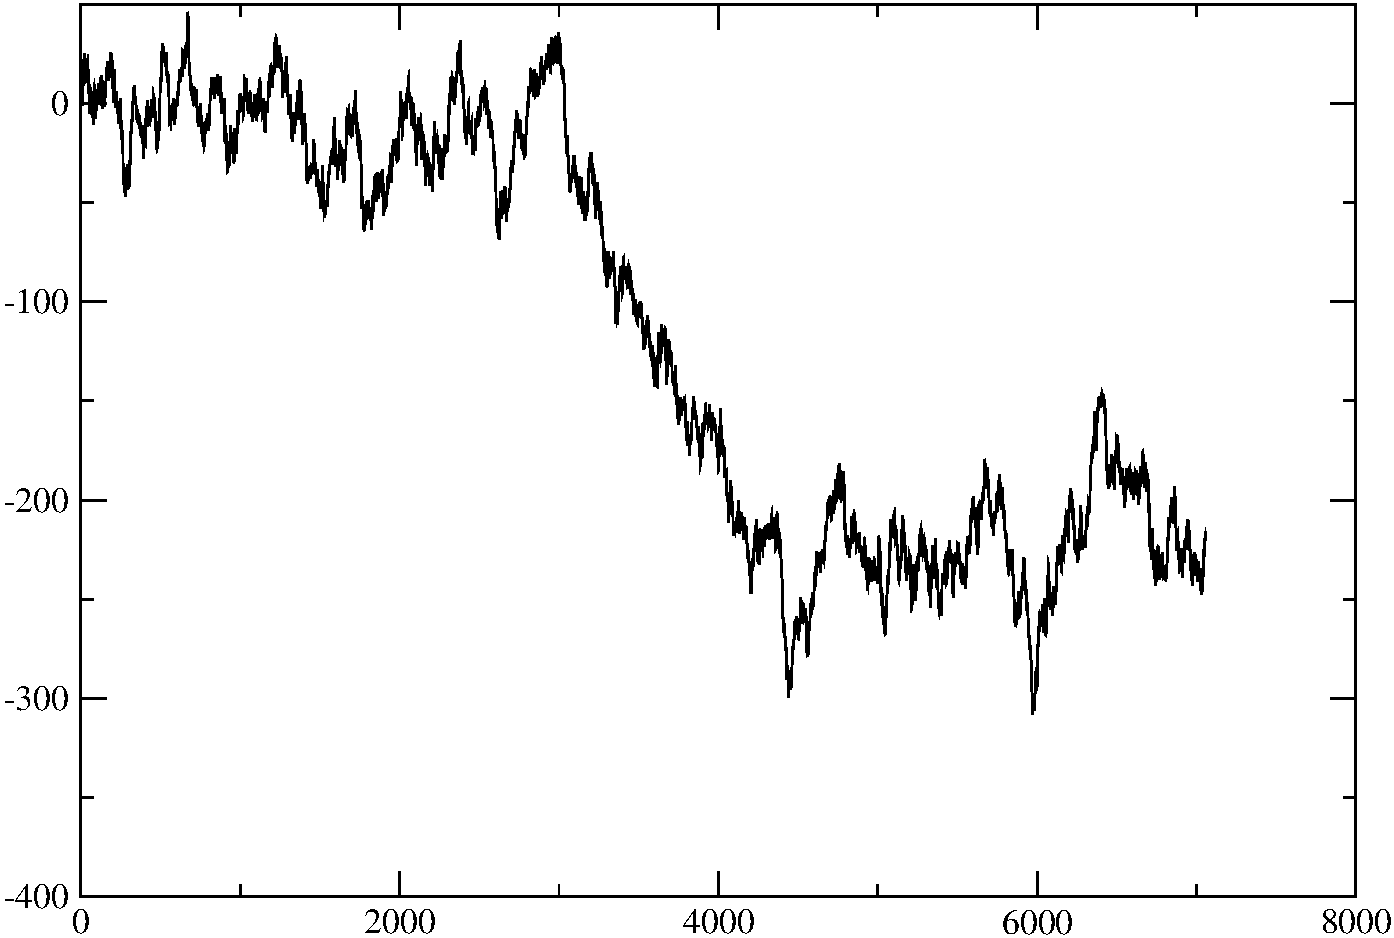
\includegraphics[width=3.5in]{figs/example.pdf}
\end{block}

\end{frame}


%===============================================================================
%     OpenMP
%===============================================================================
\begin{frame}
\frametitle{OpenMP Threading}

\begin{block}{Embarassingly Parallel}
  \begin{itemize}
  \item Each chain is completely independent
  \item Thus, each thread can run completely independent, aside from ALL\_REDUCE at end
  \item As a result, we anticipate nearly-perfect scalability. 
  \end{itemize}
\end{block}

\begin{block}{Threading the application}
  \begin{itemize}
  \item compile with: g++ test.cpp -fopenmp -lpthread
  \item OMP\_GET\_NUM\_PROCS != OMP\_GET\_MAX\_THREADS 
    \begin{itemize}
      \item Why might that be?
    \end{itemize}
  \end{itemize}
\end{block}

\end{frame}

%===============================================================================
%     Finisher!
%===============================================================================
\begin{frame}
\frametitle{Conclusions}

\begin{block}{Summary}
\begin{itemize}
  \item MCMC is a critical algorithm across a wide variety of industries and STEM fields
  \item We have demonstrated a simple C++ implementation
  \item This implementation should scale well on a single lonestar node
\end{itemize}
\end{block}

\begin{block}{Thank you!}
\begin{itemize}
\item nick@ices.utexas.edu for code
\item Have a Markovian Day!
\end{itemize}
\end{block}

\end{frame}

\end{document}
